\documentclass[12pt]{article}
\usepackage[utf8]{inputenc}
\usepackage{float} 
\usepackage{url}
%\usepackage[latin1]{inputenc}%\textbf{}
\usepackage[spanish, es-tabla]{babel} %convierte comandos en ingles al espa\~{n}ol. 
\usepackage[ ]{graphicx} %paquete para poder incluir graficas
%\DeclareGraphicsExtensions{.png,.pdf,.jpg,.jpeg,.xps}
\usepackage[right=2cm,left=3cm,top=2.5cm,bottom=2.0cm,headsep=0cm,footskip=0.5cm]{geometry} %margenes del texto
\usepackage{anysize} %Soporte para el comando de margenes
\marginsize{2cm}{2.cm}{2cm}{2cm} % Controla losmárgenes{izquierda}{derecha}{arriba}% {abajo}. 
\setlength{\parindent}{12pt}%anula la sangrí en todo el texto
\setlength{\parskip}{12pt}
\usepackage{listings}
\usepackage{color}

\definecolor{dkgreen}{rgb}{0,0.6,0}
\definecolor{gray}{rgb}{0.5,0.5,0.5}
\definecolor{mauve}{rgb}{0.58,0,0.82}

\lstset{frame=tb,
	language=Java,
	aboveskip=3mm,
	belowskip=3mm,
	showstringspaces=false,
	columns=flexible,
	basicstyle={\small\ttfamily},
	numbers=none,
	numberstyle=\tiny\color{gray},
	keywordstyle=\color{blue},
	commentstyle=\color{dkgreen},
	stringstyle=\color{mauve},
	breaklines=true,
	breakatwhitespace=true,
	tabsize=3
}

\title{\huge{\textbf{ Desarrollo de Aplicaciones para Internet: Memoria Práctica 10 }}}%Comando para el título

\author{\small \textit{{Pilar Navarro Ramírez}}}%Introducción de los nombres de los integrantes

%CUERPO DEL DOCUMENTO

\begin{document}

\maketitle
\newpage
\tableofcontents
\newpage
\section{Objetivo}
En esta última práctica de la asignatura pretendo llevar a cabo una visualización de algunos de los campos de la base de datos que usé en las prácticas anteriores. En concreto se trata de datos de los episodios de la serie de 'Friends'. Se mostrarán gráficos de líneas con las fechas de estreno de cada episodio y gráficos de barras con la duración de los distintos episodios de cada temporada. 
\section{Trabajo realizado}

Para llevar a cabo dicha visualización he usado la biblioteca \textbf{Highcharts} de JavaScript y me he basado en algunos ejemplos que aparecen en su página web, como \cite{2} y \cite{3}. 

Se puede acceder a los gráficos realizados a través del menú desplegable en la sección 'Gráficos' que aparece en la barra de navegación superior de la página principal de mi aplicación. 

\subsection{Gráficos de líneas (Line Chart)}

En primer lugar, he realizado un gráfico de líneas interactivo, con una línea por cada temporada, representando en el eje X el número del episodio y en el eje Y el año de estreno. Si se mueve el ratón sobre la línea correspondiente a cada temporada, aparece una etiqueta mostrando la fecha exacta de estreno de cada episodio y el número del mismo. Aunque no es el fin principal de este gráfico, también podemos apreciar en él el número de episodios que tiene cada temporada: una línea más larga se corresponde con una temporada con un mayor número de episodios y una línea más corta nos dice que esa temporada tiene un menor número de episodios. 

\begin{figure}[H]
	\centering
	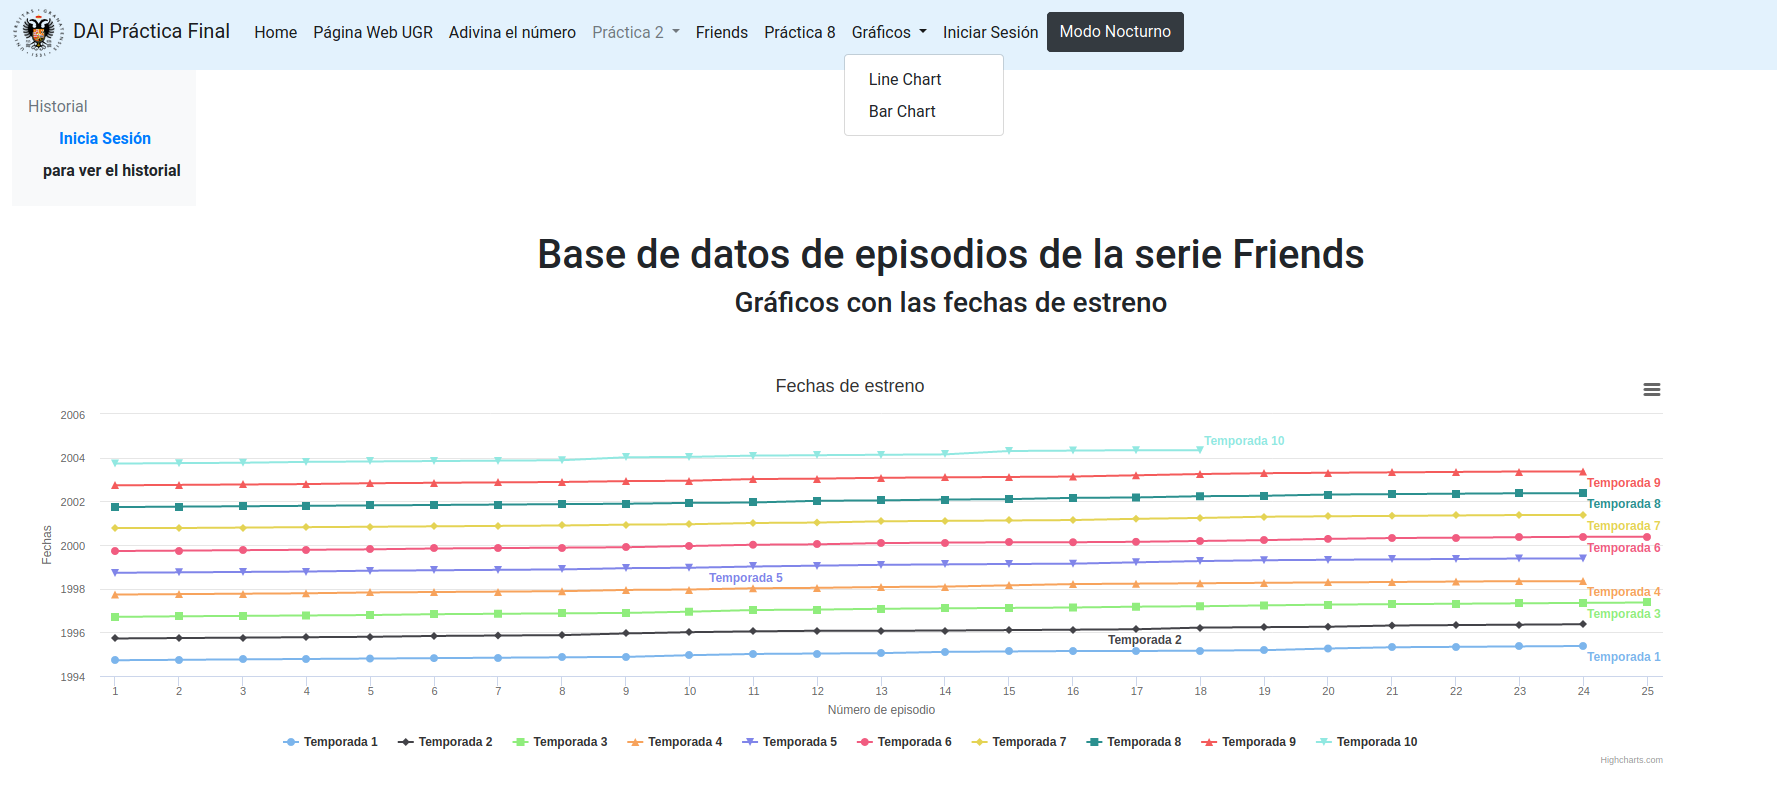
\includegraphics[width=1.1\linewidth]{captura1}
	\caption{}
	\label{fig:captura1}
\end{figure}


Con el objetivo de analizar la evolución de las fechas de estreno de las distintas temporadas, he representado otro gráfico con una sola línea que muestra las fechas de estreno del primer episodio de cada temporada. Así, en el eje X aparecen las distintas temporadas y en el eje Y el año de estreno. Como en el gráfico anterior, al mover el ratón sobre esta línea podemos ver la fecha exacta de estreno del primer episodio de cada temporada. Tras realizar dicha visualización, nos damos cuenta de que la evolución es lineal y las temporadas se han ido estrenando aproximadamente en las mismas fechas de los distintos años y con un período de tiempo similar entre las mismas. 

\begin{figure}[H]
	\centering
	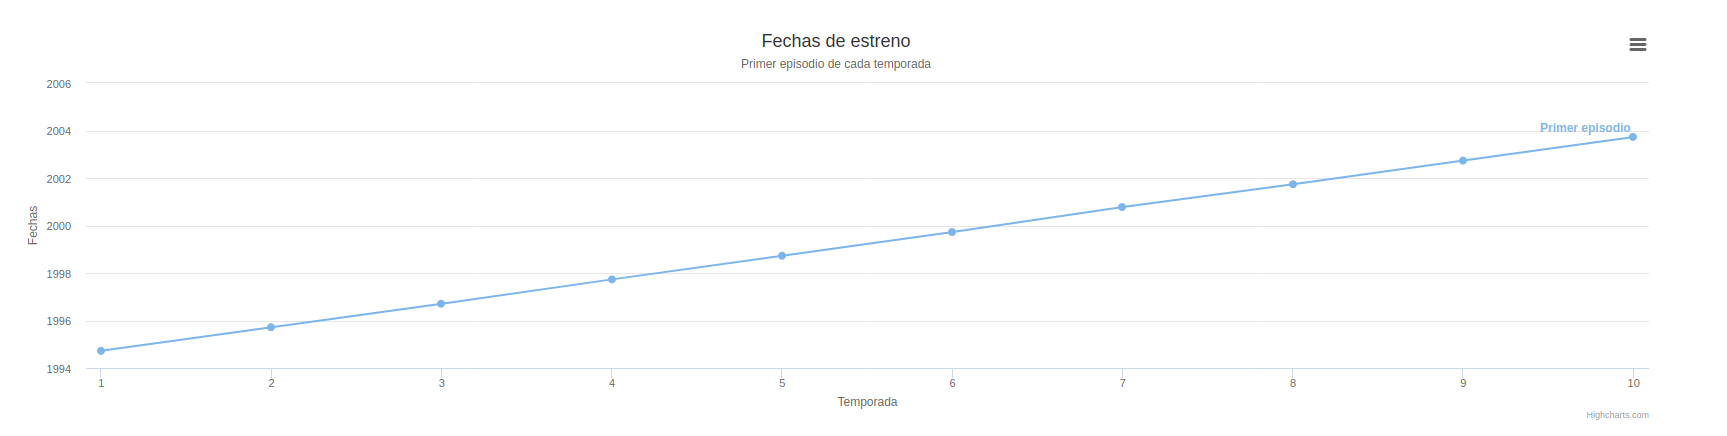
\includegraphics[width=1.1\linewidth]{captura2}
	\caption{}
	\label{fig:captura2}
\end{figure}



 El código de JavaScript correspondiente a estos gráficos se puede encontrar dentro la carpeta \textit{static}, en el archivo \textit{line\_chart.js}, y la plantilla de html para la página donde aparecen en \textit{linechart.html} en la carpeta de \textit{templates}.
 
 \subsection{Gráficos de barras (Bar Chart)}
 
 Además de los gráficos de líneas anteriores, he visualizado algunos gráficos de barras, donde se muestra la duración de los distintos episodios de cada temporada. En un primer gráfico se representa con un barra, del mismo color para la misma temporada, la duración en minutos de un episodio, para todos los episodios de todas las temporadas. En el eje X aparece el número del episodio y en el eje Y la duración en minutos. Al mover el ratón por las barras aparece una etiqueta en sobre la barra seleccionada que puesta la temporada y el episodio al que corresponde así como su duración, de manera que se puede navegar por él haciendo más fácil su interpretación. 
 \begin{figure}[H]
 	\centering
 	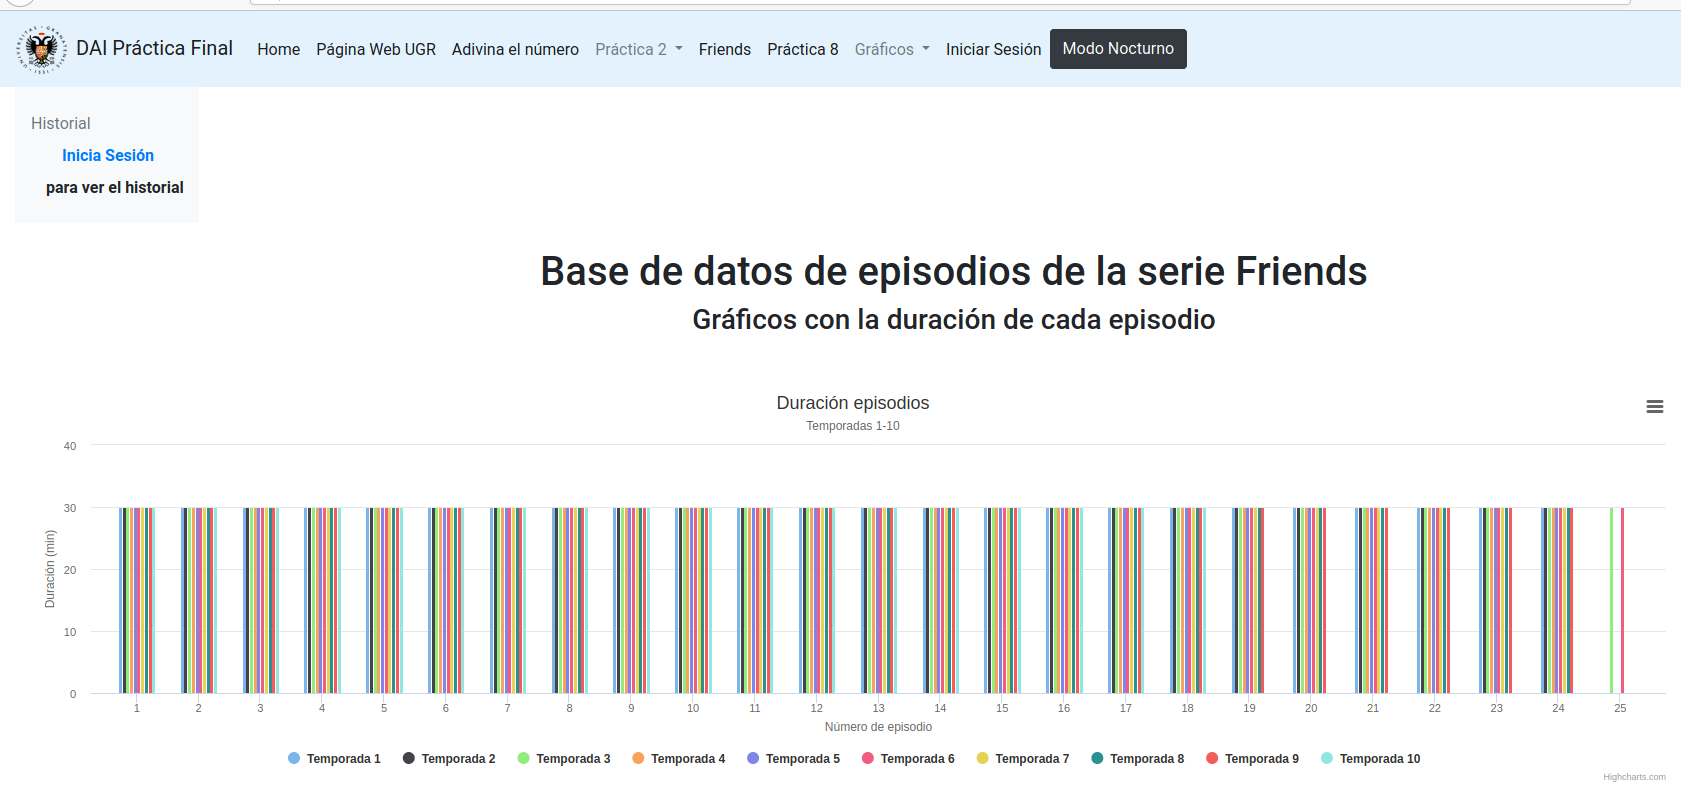
\includegraphics[width=1.1\linewidth]{captura3}
 	\caption{}
 	\label{fig:captura3}
 \end{figure}
 
 Es de notar que todos los episodios tienen exactamente la misma duración, 30 min, pero, si esta fuera diferente para cada episodio, este gráfico resultaría muy útil para comparar las duraciones de los mismos y ver si la temporada influye en la duración o no, por ejemplo (como hemos dicho no es nuestro caso por los datos tan aburridos de los que disponemos en nuestra base de datos). Además, al haber muchos episodios y muchas temporadas, las barras son más bien líneas, y es muy difícil distinguir las barras de las distintas temporadas. Por eso, he visualizado el mismo gráfico varias veces pero solo con ciertas temporadas (3 en cada gráfico) y las veces necesarias para cubrir todas las temporadas, de manera que la información sea más fácil de interpretar y agradable a la vista. 
 
 \begin{figure}[H]
 	\centering
 	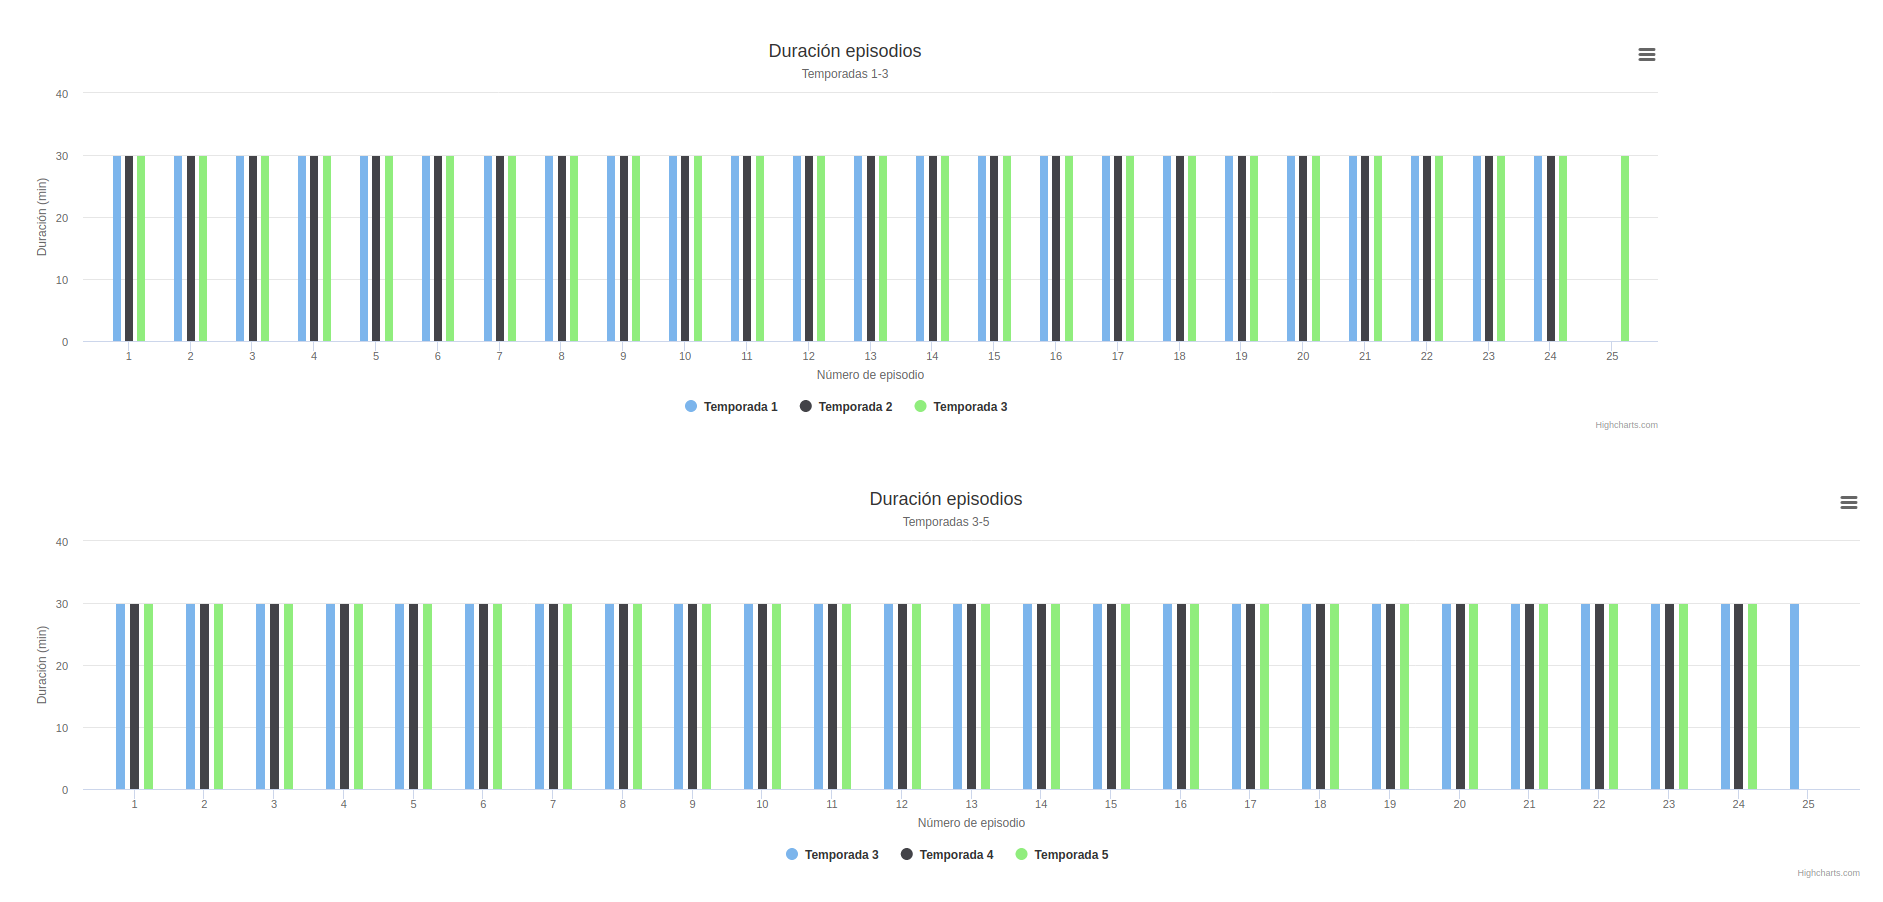
\includegraphics[width=1.1\linewidth]{captura4}
 	\caption{}
 	\label{fig:captura4}
 \end{figure}
 
  El código de JavaScript correspondiente a estos gráficos se puede encontrar dentro la carpeta \textit{static}, en el archivo \textit{bar\_chart.js}, y la plantilla de html para la página donde aparecen en \textit{barchart.html} en la carpeta de \textit{templates}.

\section{Problemas encontrados durante la implementación}
\subsection{Primer problema: Petición a la API asíncrona}
Para obtener los datos de la base de datos, hay que realizar una petición GET a la API REST que programé en la práctica 5, en concreto a la uri \textit{/api/episodios}. Implementé al principio una función (\textit{get\_dates()}) que hace dicha petición, obtiene de la respuesta las fechas de estreno de los distintos episodios de cada temporada y devuelve estas fechas. A continuación llamaba a esta función dentro de otra que implementa el gráfico y usa como datos a representar los devueltos por esta función. Sin embargo, el gráfico aparecía en blanco, porque se dibujaba antes de que la petición realizada por la primera de las funciones fuera resuelta, por lo que no disponía de datos que representar. 

Para resolver este problema decidí crear una \textbf{Promesa} asociada a la función problemática: 
\begin{lstlisting}
function get_dates() {
	return new Promise((resolve, reject) => {
		let fechas = {}
		$.getJSON('/api/episodios').done(function(respuesta) {
			$.each(respuesta, function(key, value) {
				if (!(value['season'] in fechas)) {
					fechas[value['season']] = []
				}
				fechas[value['season']].push([value['number'], Date.parse(value['airdate'])])
			});
			resolve(fechas)
		});
	})
}
\end{lstlisting}

 Esto permite que, en vez de inmediatamente retornar el valor final, la función asíncrona devuelva una promesa de suministrar el valor en algún momento en el futuro. En la función que implementa el gráfico, usé entonces el operador \textbf{await} al llamar a la función \textit{get\_dates()}, para que la ejecución se pare hasta que la Promesa termine. De esta forma, se evita que se dibuje el gráfico antes de que la petición que provee los datos sea resuelta.
 \begin{lstlisting}
async function draw_linechart() {
	let fechas = await get_dates();
 \end{lstlisting}
 
\subsection{Segundo Problema: Formato de los datos de fecha}
Tras solucionar el problema anterior, seguía obteniendo el gráfico de líneas en blanco, por lo que algo seguía yendo mal. Después de probar varias cosas llegué a la conclusión de que el problema eran las fechas, no estaban en el formato correcto. En efecto, los charts de \textbf{Highcharts} sólo aceptan fechas en formato númerico, es decir, en milisegundos desde el 1 de Enero, 1970, 00:00:00, pero las fechas de mi base de datos tenían el formato 'yyyy-mm-dd'. 

Para pasarlas al formato correcto, simplemente había que usar el método \textbf{parse()} del objeto \textbf{Date}. Y ya se veía el gráfico con todas las líneas correctamente.
\begin{lstlisting}
fechas.push([value['season'], Date.parse(value['airdate'])])
\end{lstlisting}

\subsection{Tercer Problema: Visualización del formato numérico de las fechas}

Ya tenía el gráfico, pero ahora se mostraba la fecha en las etiquetas en formato numérico, lo cual es muy poco entendible para quien vea el gráfico. Por lo tanto, decidí en primer lugar desactivar las etiquetas de los datos
\begin{lstlisting}
plotOptions: {
	line: {
		dataLabels: {
			enabled: false
	},
},
\end{lstlisting}

A continuación, investigué cómo cambiar el formato de los datos que aparecen en la etiqueta que se muestra al mover el ratón sobre los puntos del gráfico, la cual es llamada \textit{tooltip}, y fui capaz de ponerle una cabecera con la temporada y un texto con el número del episodio correspondiente al punto sobre el que se mueve el ratón y su fecha de estreno en un formato adecuado. Para ello me basé en el ejemplo \cite{7} y en los formatos de fechas que usa Highcharts \cite{8}, de manera que basta escribir lo siguiente en el código del gráfico:
\begin{lstlisting}
 tooltip: {
	headerFormat: '<b>{series.name}</b><br>',
	pointFormat: 'Episodio {point.x}:{point.y:%e. %b %Y}'
},
\end{lstlisting}
\begin{figure}[H]
	\centering
	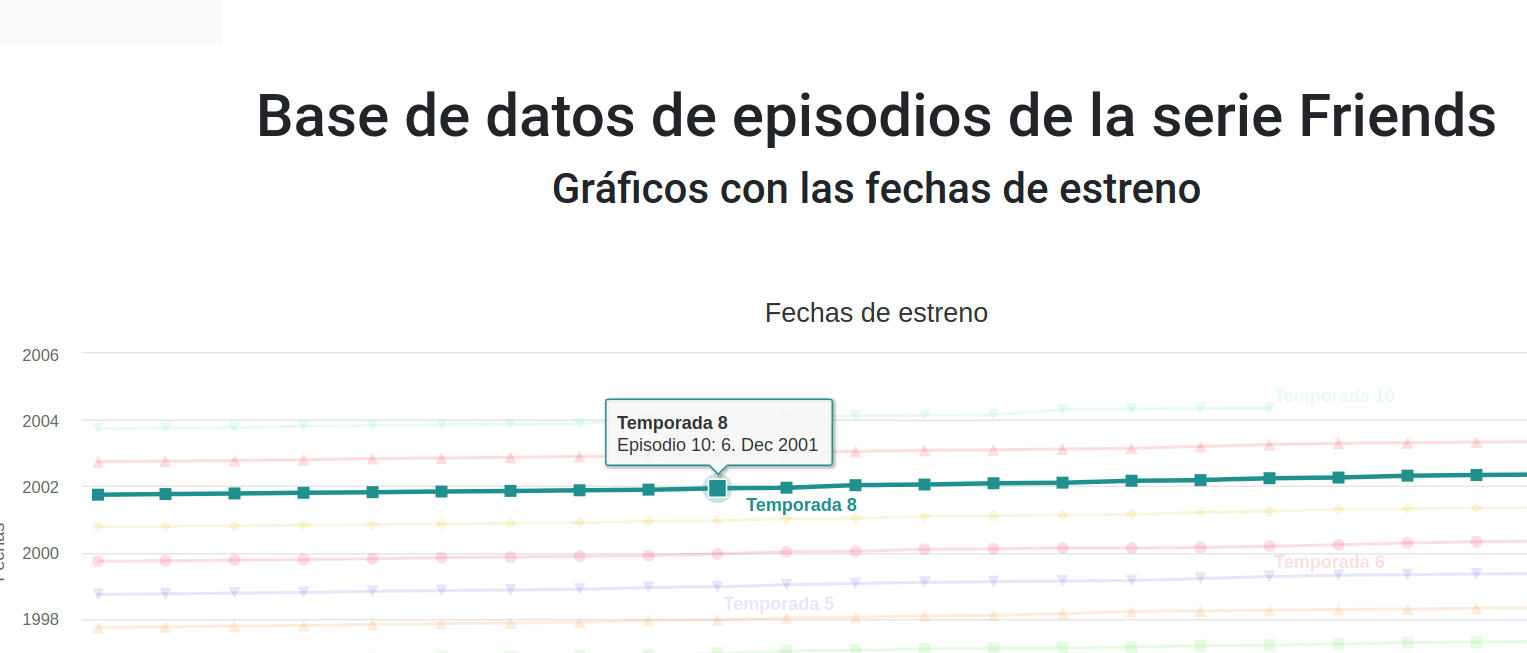
\includegraphics[width=1\linewidth]{captura5}
	\caption{}
	\label{fig:captura5}
\end{figure}

Así, el formato de fecha que aparecía en las etiquetas ya era legible, y no era necesario cambiarlo de ningún otro sitio. 

\textbf{Nota:} Estos han sido los problemas más 'graves' que me han surgido durante la realizción de la práctica y que me ha llevado más tiempo en resolver. Los demás problemas se resolvían simplemente mirando en la documentación o volviendo sobre el código para ver qué había hecho mal, qué nombre había puesto mal o qué coma me había faltado. Para los gráficos de barras, que implementé después, como ya tenía experiencia y había resuelto los problemas principales, no tuve muchas dificultades. 
\newpage
\section{Herramientas alternativas}

Otra biblioteca de JavaScript que podía haber usado para visualizar los datos es \textbf{d3.js}, que se usa para manipular documentos basado en datos y está especializada en visualización de datos en páginas web, o \textbf{c3.js} que hace uso de la primera. En \cite{11} aparecen ejemplos de gráficos con d3.js y en \cite{13} con c3.js. Su uso me parecía un poco más complicado, por eso me decidí por Highcharts. Además de estas bibliotecas, está también \textbf{chart.js}, otra biblioteca para visualicación de datos, de uso similar a Hihgcharts. Podemos ver algunos ejemplos en \cite{12}.
\newpage
\begin{thebibliography}{10}

{%apertura
\setlength{\parindent}{0cm} %Estas instrucciones anulan la sangr´\'ia en los párrafos que esten dentro de los corchetes

\bibitem{1} 
\url{https://www.highcharts.com/}

\bibitem{2} 
\url{https://www.highcharts.com/demo/line-basic}

\bibitem{3} 
\url{https://www.highcharts.com/demo/column-basic}

\bibitem{4}
\url{https://developer.mozilla.org/es/docs/Web/JavaScript/Referencia/Operadores/await}

\bibitem{5}
\url{https://developer.mozilla.org/es/docs/Web/JavaScript/Referencia/Objetos_globales/Promise}

\bibitem{6}
\url{https://developer.mozilla.org/es/docs/Web/JavaScript/Referencia/Objetos_globales/Date/parse}

\bibitem{7}
\url{https://www.highcharts.com/demo/spline-irregular-time}

\bibitem{8} 
\url{https://api.highcharts.com/highcharts/yAxis.dateTimeLabelFormats}


\bibitem{9} 
\url{https://www.highcharts.com/docs/getting-started/how-to-set-options}


\bibitem{10} 
\url{https://www.highcharts.com/docs/getting-started/your-first-chart}


\bibitem{11} 
\url{https://www.d3-graph-gallery.com/}

\bibitem{12} 
\url{https://www.chartjs.org/samples/latest/}

\bibitem{13} 
\url{https://c3js.org/examples.html}
}


\end{thebibliography}

\end{document}